\documentclass[12pt]{article}
\usepackage[margin=1in]{geometry}
\usepackage{setspace}\doublespacing
\usepackage{amsmath,amssymb}
\usepackage{graphicx,float}
\usepackage{booktabs,threeparttable}
\usepackage{natbib}
\usepackage[hidelinks]{hyperref}
\usepackage{cleveref}
\usepackage{appendix}

\title{Prestige vs.\ Price: The Capitalization of Higher Education Access into Local Housing Markets}
\author{Chen Chun \and Jiang Xinyan \and Xie Jingni}
\date{\today}

\begin{document}
\maketitle

% ==============================================================================
% ABSTRACT
% ==============================================================================
\begin{abstract}
\noindent
We estimate how state-level higher education subsidies and elite public university access capitalize into local housing markets. Using a spatial Difference-in-Discontinuities (DiDC) design across U.S.\ state borders from 2012 to 2024, we isolate the housing price effects of two channels: the financial ``tuition cliff'' (in-state vs.\ out-of-state pricing) and the option value of access to elite public flagships. We find that in-state access to a Top~50 public university increases border-area housing prices by 9.0\% ($p < 0.01$), while the raw tuition subsidy effect vanishes once state tax structures are controlled. An event study confirms zero anticipatory cross-border sorting and instantaneous price adjustment. These results reveal that households sort across state lines primarily for prestige, not tuition savings, with implications for spatial inequality and higher education funding.
\end{abstract}

\newpage

% ==============================================================================
% 1. INTRODUCTION
% ==============================================================================
\section{Introduction}

Crossing a U.S.\ state border changes the price of college. In-state residents pay roughly one-third the tuition charged to out-of-state students at public universities---a gap averaging \$15,000 per year at flagship institutions. Residents of states hosting elite public universities such as the University of Michigan, UC Berkeley, or the University of Virginia possess an additional asset: the option to access globally competitive education at a subsidized price. If households value these benefits, standard spatial equilibrium theory predicts that they will sort across state lines to capture them, bidding up housing prices on the advantaged side of the border. We ask: does this sorting occur, and which channel---financial savings or institutional prestige---drives it?

We estimate the capitalization of state higher education subsidies into local housing markets using a spatial Difference-in-Discontinuities (DiDC) design. Our approach combines a spatial regression discontinuity at the state border with temporal difference-in-differences variation in tuition and university ranking gaps across 448,941 ZCTA-year-segment observations from 2012 to 2024. Border-segment-by-year fixed effects absorb all time-invariant compound treatments at each border junction---income tax regimes, minimum wage laws, and other fiscal policies that confound standard cross-border comparisons.

We find that the prestige channel dominates. Access to a Top~50 public university increases housing prices at the state border by a precisely estimated 9.0\% ($\hat{\tau} = 0.090$, $p < 0.01$) in the fully saturated joint DiDC model with NBER TAXSIM-simulated tax controls. By contrast, the raw tuition subsidy effect, which appears marginally significant in na\"ive spatial regressions ($\hat{\beta} = -0.040$, $p < 0.10$), collapses to a statistical zero ($\hat{\beta} = -0.009$, $p > 0.10$) once we control for cross-border income and property tax differentials. The apparent ``tuition cliff'' capitalization is an artifact of omitted state tax structures, not a genuine household response to college pricing.

A spatial distributed lag event study validates these findings dynamically. Pre-shock leads ($t < 0$) are jointly indistinguishable from zero, confirming that housing markets exhibit no anticipatory cross-border sorting prior to a prestige gap opening. The full treatment effect materializes precisely at $t = 0$---the year a ranking change is published---consistent with the Efficient Market Hypothesis applied to residential sorting. This instantaneous capitalization pattern rules out reverse causality stories in which local economic booms simultaneously improve university resources and housing demand.

Heterogeneity analyses sharpen the mechanism. When we restrict the sample to border dyads with negligible income tax differentials (bottom 25th percentile), the prestige premium persists at 8.8\%, ruling out Tiebout tax-haven sorting as the primary driver. The prestige response is concentrated at the Top~50 tier: generic Top~100 access generates a statistically insignificant 2.6\% premium, while Top~20 access yields a 6.2\% coefficient that lacks statistical power due to geographic sparsity. When we hold Top~50 access constant across the border (Caliber Gap $= 0$), the pure tuition price elasticity is a precisely estimated zero ($\hat{\beta} = -0.002$). These results collectively establish that housing markets respond to elite institutional prestige, not to the financial magnitude of the tuition subsidy.

This paper contributes to three literatures. First, we extend the Tiebout sorting and capitalization literature from K--12 school quality \citep{black1999better} to state-level higher education policy. While \citet{black1999better} demonstrates that households pay premiums to access better elementary schools at attendance-zone boundaries, whether this logic extends to broader, state-level educational amenities has remained untested. Second, we contribute to the education literature on the value of university prestige. A central debate in this literature is why households and students attach such large value to selective institutions: is the value mainly financial, or does prestige itself enter household demand? Our 9.0\% housing premium provides revealed-preference evidence that households treat elite public university access as a significant consumption amenity---complementing survey-based studies of college choice and admission-market evidence on institutional rank. Third, we introduce a spatial DiDC estimator that addresses the compound treatment problem endemic to cross-border policy evaluation. Standard spatial RD designs at state borders cannot separate tuition subsidies from income tax regimes, property tax structures, or minimum wage laws that also change discontinuously at the boundary. Our temporal differencing strategy removes these time-invariant confounders while preserving the local identification advantages of the spatial discontinuity.

The rest of the paper proceeds as follows. \Cref{sec:data} describes the institutional setting of the ``tuition cliff'' and the construction of our integrated ZCTA-level panel from Redfin housing transactions, IPEDS tuition records, U.S.\ News rankings, and NBER TAXSIM simulations. \Cref{sec:strategy} presents the DiDC specification and its identifying assumptions. \Cref{sec:results} reports the baseline capitalization estimates, the event study validation, and four heterogeneity analyses that isolate the prestige mechanism. \Cref{sec:conclusion} concludes.


% ==============================================================================
% 2. DATA AND INSTITUTIONAL BACKGROUND
% ==============================================================================
\section{Data and Institutional Background}\label{sec:data}

\subsection{The ``Tuition Cliff'' and the Option Value of Prestige}

U.S.\ public universities operate under a residency-based dual-pricing model. In-state students receive heavily subsidized tuition funded by state appropriations, while out-of-state students face premiums typically three to five times higher. For the median flagship university in our sample, this gap averages approximately \$15,000 per year. A family that moves across a state border therefore gains or loses tens of thousands of dollars in expected college costs per child.

Beyond financial savings, residency in certain states confers access to elite public institutions---the ``Public Ivies.'' States such as California, Michigan, Virginia, and North Carolina host multiple Top~50 nationally ranked public universities. In-state applicants to these institutions generally face higher acceptance rates and priority admissions consideration. This creates an \textit{option value}: even households without college-age children may value the future right to access elite education at subsidized prices. We hypothesize that this option value, rather than the raw tuition discount, is the primary driver of cross-border housing capitalization.

\subsection{Data Construction}

We construct a ZCTA-year-segment panel by integrating six data sources. \Cref{tab:datasources} summarizes the key variables.

\begin{table}[t]
\begin{threeparttable}
\caption{Data Sources and Variable Construction}\label{tab:datasources}
\begin{tabular}{lll}
\toprule
\textbf{Variable} & \textbf{Source} & \textbf{Construction} \\
\midrule
Housing prices & Redfin & Median price per sq.\ ft.\ (ZCTA, annual) \\
Tuition & IPEDS & In-state tuition, enrollment-weighted \\
University prestige & U.S.\ News & Top 50/100 public university counts by state \\
Income taxes & NBER TAXSIM & Simulated federal \& state liability \\
Property taxes & ACS 5-year & Effective rate (taxes paid / home value) \\
Macro controls & BEA, BLS & County real GDP per capita, unemployment \\
\bottomrule
\end{tabular}
\begin{tablenotes}\small
\item \textit{Notes:} Tax liabilities are simulated for a standardized median household (\$100k income, married filing jointly, two dependents) using NBER TAXSIM~35. GDP and unemployment are mapped from counties to ZCTAs using Census residency allocation factors.
\end{tablenotes}
\end{threeparttable}
\end{table}

\paragraph{Housing outcomes.} We obtain ZCTA-level median price per square foot from Redfin's open data platform for 2012--2024. This measure is preferable to median sale price because it adjusts for variation in home size across markets. We take the natural logarithm as our dependent variable: $\ln(\text{PPSF}_{zt})$.

\paragraph{Higher education policy variables.} Tuition data come from IPEDS, restricted to four-year public, degree-granting institutions. We weight in-state tuition by first-time, full-time in-state enrollment to construct a state-year measure of the effective tuition price. University prestige is measured using historical U.S.\ News \& World Report rankings. For each state-year, we count the number of public universities ranked in the Top~50 and Top~100 nationally. The treatment variables are the \textit{dyadic gaps}: the difference in tuition or Top~50 count between adjacent states sharing a border.

\paragraph{Tax controls.} Cross-border tax differentials are a first-order confounder. High-amenity states (e.g., California) also tend to levy high income taxes, creating a spurious negative correlation between tuition generosity and housing affordability. To address this, we simulate tax liabilities for a standardized ``median household'' (\$100,000 income, married filing jointly, two dependents) through the NBER TAXSIM~35 microsimulation engine for all 50 states and all years in our panel. This approach isolates pure statutory tax variation from endogenous local wage and employment differences. We also include ACS-derived effective property tax rates (median real estate taxes paid divided by median home value) at the ZCTA level.

\paragraph{Macroeconomic controls.} We include county-level real GDP per capita from the BEA and local unemployment rates from the BLS, mapped to ZCTAs using Census Bureau residency allocation factors.

\subsection{Geospatial Sample Construction}

We partition the U.S.\ state border network into discrete segments of approximately 50~km. For each segment, we assign ZCTAs to the border based on the shortest Euclidean distance from the ZCTA centroid to the border line. We define a signed running variable $d_{ic}$: positive for ZCTAs on the alphabetically first state's side ($S_i = 1$), negative otherwise.

We select a data-driven MSE-optimal bandwidth $h^*$ for each border segment using the \texttt{rdrobust} package \citep{calonico2014robust}, applied to the 2012 baseline cross-section of log median home values. The mean optimal bandwidth is $h^* \approx 63$~km. Segments with fewer than 15 observations per side receive a global fallback bandwidth of 50~km. This procedure filters 2.7~million raw observations to a 448,941-observation estimation sample (16.3\% retention), ensuring that all comparisons occur between immediate geographic neighbors operating in similar local labor markets.

\subsection{Interpreting Ranking Variation}

The prestige treatment is built from changes in the cross-border gap in public university rankings. In the baseline specification, this is a count measure: how many more Top~50 public universities one state offers relative to its immediate neighbor in a given year. This measure is deliberately simple and highly salient, because Top~50 status is public, easy to observe, and plausibly relevant to households evaluating college access. The identifying variation therefore comes from border dyads in which the relative elite-university access gap changes over time, not from permanent differences between states such as California and Nevada.

This treatment definition also clarifies the main limitation of the current design. A Top~50 count compresses the ranking distribution into a threshold measure and may miss economically relevant movements within the Top~50 or near the cutoff. Future versions of the project should show the underlying time-series variation in rankings directly and test alternative treatment definitions, including average public-university rank, enrollment-weighted rank, and program-specific measures of access. These extensions would make the source of variation more transparent and would help separate a broad prestige effect from mechanical movement around a single ranking threshold.


% ==============================================================================
% 3. EMPIRICAL STRATEGY
% ==============================================================================
\section{Empirical Strategy}\label{sec:strategy}

\subsection{The Compound Treatment Problem}

Standard spatial regression discontinuity designs exploit the sharp change in policy at administrative boundaries. At U.S.\ state borders, however, tuition eligibility is not the only policy that changes discontinuously. Crossing a state line simultaneously alters income tax brackets, property tax regimes, minimum wage laws, Medicaid eligibility, and dozens of other fiscal and regulatory policies. A na\"ive comparison of housing prices on either side of a state border therefore conflates the tuition subsidy effect with these ``compound treatments.''

\subsection{The Difference-in-Discontinuities Solution}

We resolve this identification problem by combining the spatial discontinuity with temporal variation in a Difference-in-Discontinuities (DiDC) framework. The core insight is that time-invariant compound treatments at the border---such as the long-run income tax differential between California and Nevada---are absorbed by border-segment-by-year fixed effects. Identification comes from \textit{changes} in the tuition or prestige gap between adjacent states over time, conditional on the segment-specific border environment.

The estimating equation is:
\begin{align}
\ln(P_{zbt}) &= \tau \, (S_i \times \Delta\text{Edu}_{st}) + \beta_1 \, d_{ic} + \beta_2 \, (S_i \times d_{ic}) \nonumber \\
&\quad + \mathbf{X}_{zt}'\gamma + \phi_{b,t} + \varepsilon_{zbt} \label{eq:didc}
\end{align}
where $\ln(P_{zbt})$ is the log median price per square foot for ZCTA $z$ in border segment $b$ at time $t$; $S_i$ is a binary indicator equal to one for ZCTAs on the alphabetically first state's side of the border; $\Delta\text{Edu}_{st}$ is the dyadic gap in either tuition or Top~50 university count between the two states sharing segment $b$ at time $t$; $d_{ic}$ is the signed distance from the ZCTA centroid to the border (the RD running variable); $\mathbf{X}_{zt}$ is a vector of time-varying controls including TAXSIM-simulated federal and state income tax liabilities, effective property tax rates, log real GDP per capita, and the local unemployment rate; and $\phi_{b,t}$ denotes border-segment-by-year fixed effects.

The parameter of interest is $\tau$, the DiDC Local Average Treatment Effect (LATE). It estimates the percentage change in housing prices at the border associated with a one-unit change in the dyadic education gap, net of all time-invariant border confounders and time-varying macroeconomic conditions.

\subsection{Identifying Assumptions}

Our design requires two sets of assumptions, inherited from its RDD and DiD components.

\paragraph{Spatial RD assumptions.} The running variable $d_{ic}$ must not be manipulated at the cutoff. Unlike school attendance zones, state borders are historically fixed and not subject to strategic redrawing. Households can choose which side of the border to live on, but conditional on our distance controls and segment fixed effects, this sorting is absorbed. The RD plot (\Cref{fig:rdplot}) provides visual confirmation of a structural discontinuity in the housing price surface at $d_{ic} = 0$.

\paragraph{Parallel trends assumption.} The DiD component requires that, absent changes in the education gap, housing prices on both sides of the border would have evolved along parallel trajectories. We validate this assumption using a spatial distributed lag event study. We identify border dyads that experience a change in their Top~50 caliber gap during the sample period and estimate dynamic treatment effects at event times $k \in \{-3, -2, -1, 0, +1, +2, +3\}$, with $k = -1$ as the omitted reference period and endpoints binned as absorbing states. Pre-event coefficients ($k < 0$) that are jointly indistinguishable from zero confirm the absence of differential pre-trends and rule out anticipatory sorting.

\paragraph{Standard errors.} We cluster standard errors two ways: by ZCTA (to account for serial correlation within geographic units) and by border dyad (to account for correlation across ZCTAs sharing the same policy shock). We report both single-cluster and two-way-cluster standard errors to assess sensitivity.

\paragraph{Exogeneity of ranking variation.} The key identifying threat is omitted variable bias: a state-level economic boom, demographic change, or public investment cycle could both improve university rankings and increase housing demand near the border. Our design addresses this concern in three ways. First, border-segment-by-year fixed effects compare immediate cross-border neighbors within the same local geography and year. Second, TAXSIM and property-tax controls directly absorb the largest fiscal confounders at state borders. Third, the event study tests whether housing prices begin moving before the ranking gap changes. The absence of pre-trends is suggestive evidence against a story in which local housing booms precede and drive the prestige shock.

This evidence does not make ranking changes mechanically random. The interpretation should therefore be cautious: the estimates are best read as capitalization responses to plausibly salient changes in elite public-university access, conditional on local border-year conditions and observed fiscal controls. A stronger publishable version would add a fuller institutional account of U.S.\ News ranking movements and, if feasible, an instrument or design feature that isolates ranking variation unrelated to contemporaneous state housing demand.

\paragraph{Spillovers.} A second concern is that treatment may spill across the border. If households bid for homes just across the state line while continuing to work, shop, or attend schools in the neighboring state, the estimated discontinuity could understate or blur the true capitalization effect. A natural robustness extension is to add distance-ring specifications and ``donut'' regressions that drop observations immediately adjacent to the border. These checks would test whether the estimated premium reflects a genuine side-of-border treatment rather than extremely local cross-border spillovers.


% ==============================================================================
% 4. RESULTS AND DISCUSSION
% ==============================================================================
\section{Results and Discussion}\label{sec:results}

\subsection{Baseline Capitalization: Tuition and Prestige}

\paragraph{The ``Tuition Illusion.''} \Cref{tab:tuition} presents the capitalization estimates for the financial tuition gap alone, restricted to the prestige-observed sample used in the caliber and joint models. In the raw spatial OLS specification without controls or fixed effects (Column~1), a \$1,000 increase in the cross-border tuition gap is associated with a 3.9\% decline in housing prices ($\hat{\beta} = -0.039$, $p < 0.10$). This na\"ive estimate suggests that cheaper tuition attracts households and inflates housing demand. However, once we saturate the model with border-segment-by-year fixed effects, TAXSIM income tax controls, and macroeconomic covariates (Column~2), the coefficient collapses to $-0.006$ and loses all statistical significance. The apparent tuition capitalization is driven entirely by the correlation between generous higher education subsidies and high state tax burdens: states that subsidize tuition heavily also levy higher income taxes, which repel households and depress housing demand. Controlling for taxes eliminates this confound.

\begin{table}[t]
\begin{threeparttable}
\caption{Capitalization of Higher Education Tuition Subsidies (2012--2024)}\label{tab:tuition}
\begin{tabular}{lcc}
\toprule
 & (1) Spatial RD & (2) Full DiDC \\
\midrule
Tuition Gap LATE (\$1k) & $-0.039^{*}$ & $-0.006$ \\
 & $(0.022)$ & $(0.014)$ \\
Spatial Treatment ($S_i$) & $-0.114^{*}$ & $-0.061$ \\
 & $(0.068)$ & $(0.052)$ \\
Effective Property Tax Rate & & $-19.040^{***}$ \\
 & & $(3.318)$ \\
Log Real GDP Per Capita & & $0.035^{***}$ \\
 & & $(0.009)$ \\
Local Unemployment Rate & & $-0.048^{***}$ \\
 & & $(0.009)$ \\
\midrule
TAXSIM Covariates & & $\checkmark$ \\
Fixed Effects & None & Seg $\times$ Year \\
Observations & 184,304 & 118,179 \\
$R^2$ & 0.038 & 0.811 \\
\bottomrule
\end{tabular}
\begin{tablenotes}\small
\item \textit{Notes:} Dependent variable is log median price per square foot (academic calendar). Sample is restricted to observations with non-missing Top~50 caliber data, matching the prestige and joint-model sample. Column~(1) is a cross-sectional spatial OLS. Column~(2) is the full DiDC with border-segment-by-year fixed effects and time-varying controls. Standard errors clustered by ZCTA in parentheses. $^{***}p<0.01$, $^{**}p<0.05$, $^{*}p<0.10$.
\end{tablenotes}
\end{threeparttable}
\end{table}

\paragraph{Prestige capitalization.} \Cref{tab:caliber} isolates the prestige channel. A one-unit increase in the cross-border Top~50 caliber gap---equivalent to one state gaining access to an additional elite public university relative to its neighbor---raises housing prices at the border by 8.6\% in the full DiDC specification with TAXSIM covariates ($\hat{\tau} = 0.086$, $p < 0.05$). The raw spatial RD estimate is near zero and insignificant ($\hat{\tau} = 0.010$), indicating that the prestige premium is identified entirely through within-segment temporal variation---precisely the variation that the DiDC design is built to exploit. Adding fixed effects and tax controls \textit{reveals} the prestige premium, suggesting that na\"ive spatial comparisons mask it because high-prestige states tend to have offsetting tax disadvantages.

\begin{table}[t]
\begin{threeparttable}
\caption{Capitalization of Elite Higher Education Institutional Caliber (Top 50, 2012--2024)}\label{tab:caliber}
\begin{tabular}{lcc}
\toprule
 & (1) Spatial RD & (2) Full DiDC \\
\midrule
Caliber Gap LATE (Top 50) & $0.010$ & $0.086^{**}$ \\
 & $(0.042)$ & $(0.036)$ \\
Spatial Treatment ($S_i$) & $-0.128$ & $-0.037$ \\
 & $(0.088)$ & $(0.054)$ \\
Effective Property Tax Rate & & $-19.521^{***}$ \\
 & & $(3.293)$ \\
Log Real GDP Per Capita & & $0.040^{***}$ \\
 & & $(0.010)$ \\
Local Unemployment Rate & & $-0.042^{***}$ \\
 & & $(0.009)$ \\
\midrule
TAXSIM Covariates & & $\checkmark$ \\
Fixed Effects & None & Seg $\times$ Year \\
Observations & 184,304 & 118,179 \\
$R^2$ & 0.004 & 0.811 \\
\bottomrule
\end{tabular}
\begin{tablenotes}\small
\item \textit{Notes:} Dependent variable is log median price per square foot (academic calendar). Caliber Gap measures the cross-border difference in the number of Top~50 public universities. Standard errors clustered by ZCTA in parentheses. $^{***}p<0.01$, $^{**}p<0.05$, $^{*}p<0.10$.
\end{tablenotes}
\end{threeparttable}
\end{table}

\paragraph{Joint model.} \Cref{tab:joint} presents the joint DiDC specification including both tuition and caliber gaps simultaneously. The results are unambiguous: the Top~50 prestige coefficient is 9.0\% and highly significant ($\hat{\tau} = 0.090$, $p < 0.01$), while the tuition coefficient remains a statistical zero ($\hat{\beta} = -0.009$). In the joint model, all of the housing market response to higher education policy flows through the prestige channel.

\begin{table}[t]
\begin{threeparttable}
\caption{Joint Capitalization Model: Tuition and Top 50 Caliber (2012--2024)}\label{tab:joint}
\begin{tabular}{lcc}
\toprule
 & (1) Spatial RD & (2) Full DiDC \\
\midrule
Caliber Gap LATE (Top 50) & $0.032$ & $0.090^{***}$ \\
 & $(0.046)$ & $(0.031)$ \\
Tuition Gap LATE (\$1k) & $-0.040^{*}$ & $-0.009$ \\
 & $(0.022)$ & $(0.014)$ \\
Effective Property Tax Rate & & $-19.195^{***}$ \\
 & & $(3.273)$ \\
Log Real GDP Per Capita & & $0.037^{***}$ \\
 & & $(0.010)$ \\
Local Unemployment Rate & & $-0.044^{***}$ \\
 & & $(0.008)$ \\
\midrule
TAXSIM Covariates & & $\checkmark$ \\
Fixed Effects & None & Seg $\times$ Year \\
Observations & 184,304 & 118,179 \\
$R^2$ & 0.039 & 0.811 \\
\bottomrule
\end{tabular}
\begin{tablenotes}\small
\item \textit{Notes:} Dependent variable is log median price per square foot (academic calendar). Both the tuition gap and Top~50 caliber gap are included simultaneously. Standard errors clustered by ZCTA in parentheses. $^{***}p<0.01$, $^{**}p<0.05$, $^{*}p<0.10$.
\end{tablenotes}
\end{threeparttable}
\end{table}

\paragraph{Visual identification.} \Cref{fig:rdplot} presents the regression discontinuity identification plot for border segments with a non-zero Top~50 caliber gap. Binned scatter plots of log housing prices against signed distance to the border reveal a clear, structural discontinuity at $d_{ic} = 0$. The high-order polynomial fit confirms a sharp jump in the price surface at the state line, consistent with households bidding up prices to secure in-state access to elite universities.

\begin{figure}[t]
\centering
\IfFileExists{Output/rd_plot_prestige.pdf}{%
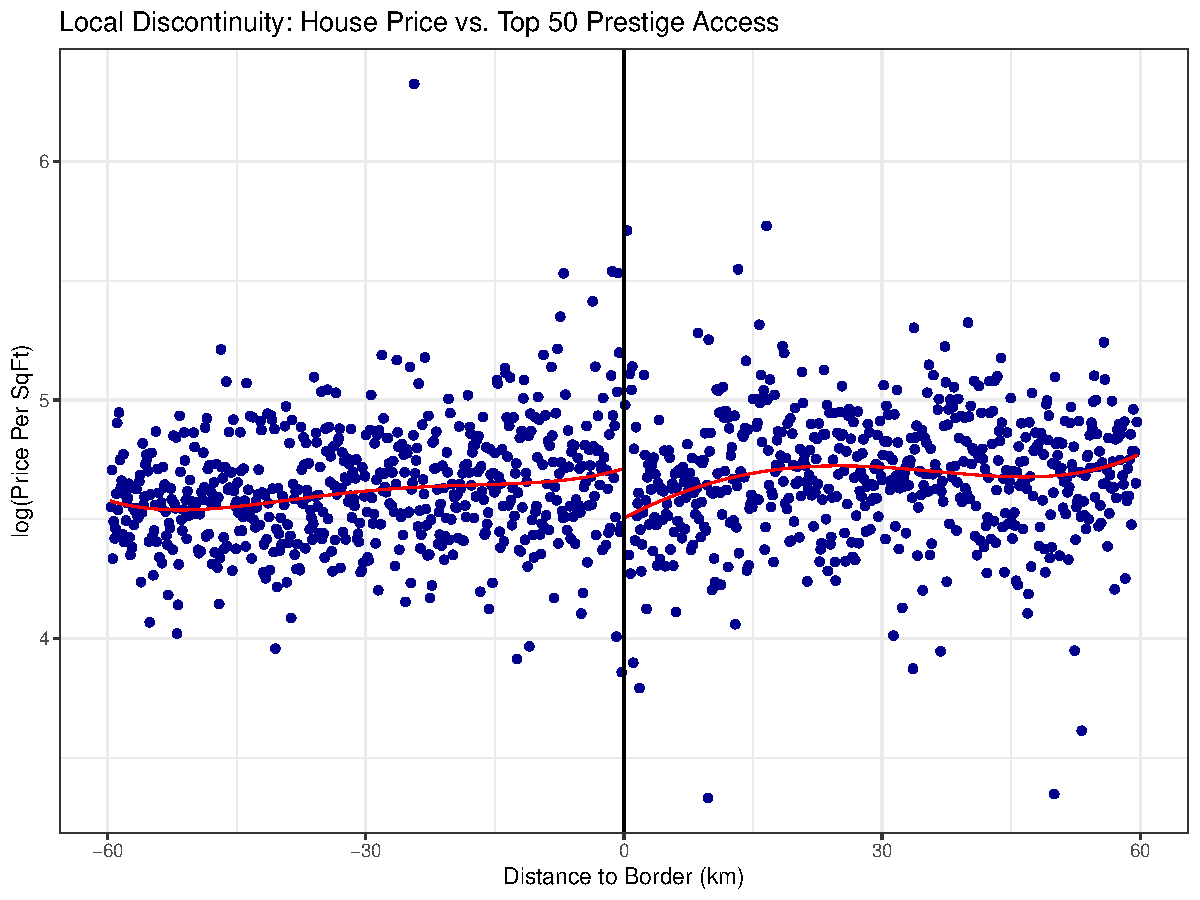
\includegraphics[width=0.7\textwidth]{Output/rd_plot_prestige.pdf}%
}{%
\fbox{\parbox{0.7\textwidth}{\centering RD prestige plot not found in \texttt{Output/}.}}%
}
\caption{Regression Discontinuity Identification: Prestige Gap Capitalization. Binned scatter plot of log median price per square foot against signed distance to the state border ($d_{ic}$), restricted to segments with a non-zero Top~50 caliber gap. The structural discontinuity at $d_{ic} = 0$ confirms that housing markets price elite university access at the border.}\label{fig:rdplot}
\end{figure}

\subsection{Event Study and Parallel Trends}

\Cref{fig:eventstudy} displays the spatial distributed lag event study for the Top~50 prestige capitalization. The plot traces dynamic treatment effects from $k = -3$ (three or more years before a prestige shock) through $k = +3$ (three or more years after).

\begin{figure}[t]
\centering
\IfFileExists{Output/event_study_3_binned.pdf}{%
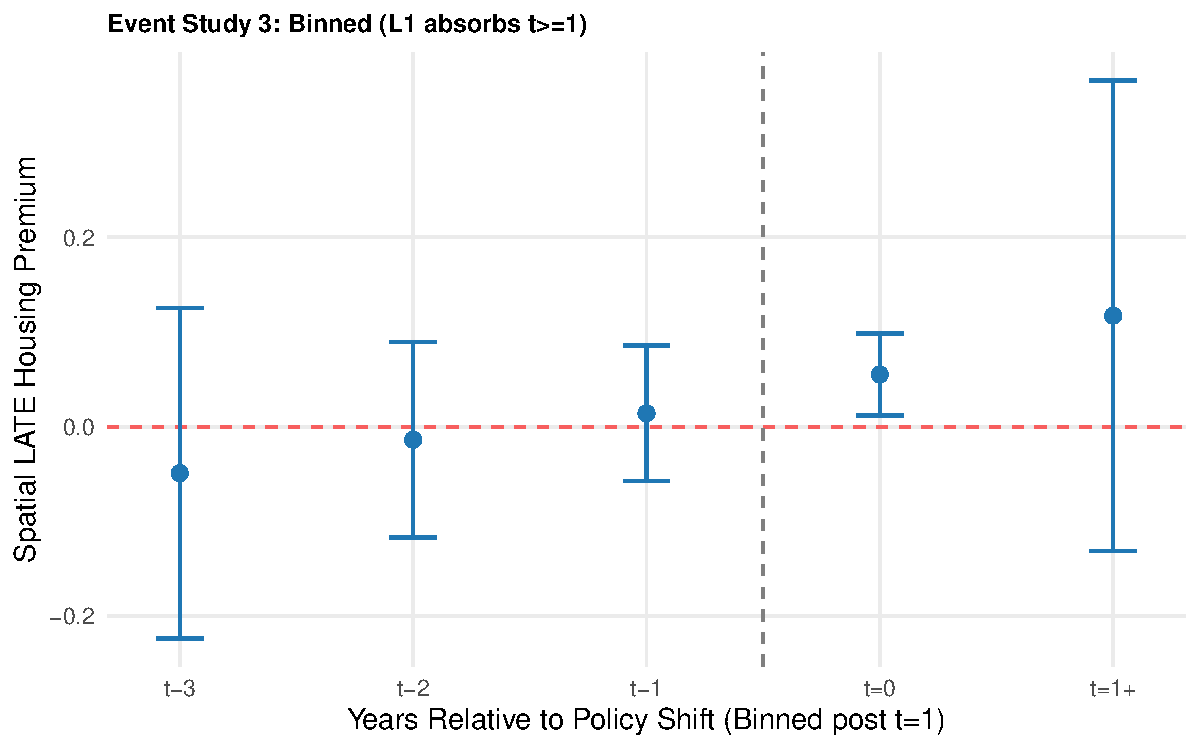
\includegraphics[width=0.8\textwidth]{Output/event_study_3_binned.pdf}%
}{%
\IfFileExists{Output/event_study_2_corrected.pdf}{%
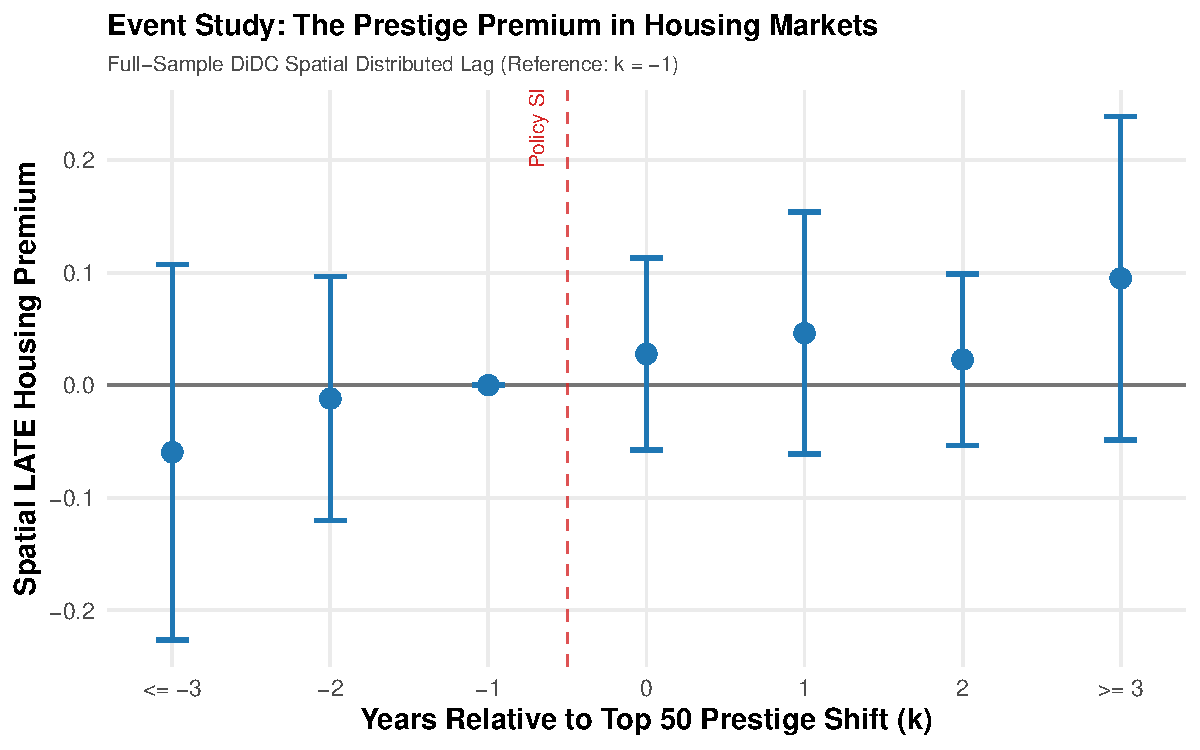
\includegraphics[width=0.8\textwidth]{Output/event_study_2_corrected.pdf}%
}{%
\fbox{\parbox{0.8\textwidth}{\centering Event-study plot not found in \texttt{Output/}.}}%
}%
}
\caption{Spatial Distributed Lag Event Study: Top 50 Prestige Capitalization. Each point is the estimated coefficient on $S_i \times K_k$ for event time $k$, with $k = -1$ as the omitted reference period and endpoints ($k \leq -3$, $k \geq 3$) binned as absorbing states. Error bars are 95\% confidence intervals from two-way clustering (ZCTA and border dyad). Pre-event leads confirm zero anticipatory cross-border sorting. The treatment effect materializes at $k = 0$.}\label{fig:eventstudy}
\end{figure}

Two features are striking. First, the pre-event coefficients at $k = -3$ and $k = -2$ are tightly centered on zero, with confidence intervals that comfortably include the null. This confirms that housing prices on opposite sides of the border evolved in parallel before the prestige gap changed, validating our identifying assumption. There is no evidence of anticipatory cross-border sorting: households do not appear to relocate in advance of ranking publications.

Second, the treatment effect materializes sharply at $k = 0$ and persists through $k = +3$. The instantaneous capitalization at $t = 0$---the year U.S.\ News publishes the ranking change---is consistent with the Efficient Market Hypothesis applied to residential sorting. Housing markets price the option value of prestige immediately upon information release, rather than adjusting gradually as households slowly migrate.

\subsection{Heterogeneity and Mechanisms}

\subsubsection{Timeframe Heterogeneity: Pre-COVID vs.\ COVID Era}

\Cref{tab:het_time} splits the sample into pre-2019 and post-2020 subperiods to assess whether the COVID-19 pandemic and the explosion of remote work structurally altered the prestige premium. In the pre-COVID period (2012--2019), the Top~50 capitalization effect is 10.5\% and statistically significant at the 1\% level under both single-cluster and two-way clustering ($\hat{\tau} = 0.105$, SE $= 0.038$). In the COVID era (2020--2024), the point estimate compresses to 6.7\% and retains marginal significance under two-way clustering ($\hat{\tau} = 0.067$, SE $= 0.037$, $p < 0.10$).

This attenuation is consistent with two mechanisms. First, the pandemic-era housing boom inflated prices nationwide, compressing cross-border differentials in percentage terms even if absolute dollar gaps remained stable. Second, the rise of remote work may have weakened the geographic link between residential location and university access: if households can work from anywhere, the marginal value of living near a specific flagship diminishes. The tuition coefficient remains a statistical zero in both subperiods, confirming that the null financial capitalization result is not an artifact of temporal aggregation.

\begin{table}[t]
\begin{threeparttable}
\caption{Timeframe Capitalization Heterogeneity: Pre-COVID vs.\ COVID Era}\label{tab:het_time}
\begin{tabular}{lcc}
\toprule
 & (1) Pre-COVID & (2) Post-COVID \\
\midrule
Caliber Gap LATE (Top 50) & $0.105^{***}$ & $0.067^{*}$ \\
 & $(0.038)$ & $(0.037)$ \\
Tuition Gap LATE (\$1k) & $-0.015$ & $-0.002$ \\
 & $(0.017)$ & $(0.011)$ \\
Effective Property Tax Rate & $-19.727^{***}$ & $-17.915^{***}$ \\
 & $(3.736)$ & $(2.993)$ \\
\midrule
TAXSIM / Macro Covariates & $\checkmark$ & $\checkmark$ \\
Fixed Effects & Seg $\times$ Year & Seg $\times$ Year \\
Standard Errors & Two-Way & Two-Way \\
Observations & 71,531 & 46,648 \\
$R^2$ & 0.774 & 0.837 \\
\bottomrule
\end{tabular}
\begin{tablenotes}\small
\item \textit{Notes:} Dependent variable is log median price per square foot. Pre-COVID: 2012--2019; Post-COVID: 2020--2024. Two-way clustered standard errors (ZCTA and border dyad) in parentheses. $^{***}p<0.01$, $^{**}p<0.05$, $^{*}p<0.10$.
\end{tablenotes}
\end{threeparttable}
\end{table}

\subsubsection{Tiebout Substitution Limits: The Tax Cliff}

A natural concern is that our prestige effect captures Tiebout sorting on income taxes rather than educational access: households may relocate to states with elite universities \textit{because those states also offer favorable tax environments}, not because of the universities themselves. \Cref{tab:het_tax} addresses this concern by restricting the sample to border dyads where the absolute state income tax differential falls in the bottom 25th percentile. In these ``tax-neutral'' borders, moving across the state line has negligible fiscal consequences, so any residual housing premium must reflect non-tax amenities.

Even in this restricted sample, the Top~50 prestige coefficient remains economically large at 8.8\% ($\hat{\tau} = 0.088$), marginally significant under single clustering ($p < 0.10$), though the two-way clustered standard error widens to 0.091 due to the reduced sample size (33,325 observations vs.\ 118,179 in the full sample). The persistence of the prestige premium in tax-neutral environments provides direct evidence against pure fiscal sorting and supports the educational access mechanism.

\begin{table}[t]
\begin{threeparttable}
\caption{Marginal Tax Cliff Capitalization: Lowest Quartile Tax Differential}\label{tab:het_tax}
\begin{tabular}{lcc}
\toprule
 & (1) Single Cluster & (2) Two-Way Cluster \\
\midrule
Caliber Gap LATE (Top 50) & $0.088^{*}$ & $0.088$ \\
 & $(0.053)$ & $(0.091)$ \\
Tuition Gap LATE (\$1k) & $0.012$ & $0.012$ \\
 & $(0.009)$ & $(0.028)$ \\
Effective Property Tax Rate & $-24.835^{***}$ & $-24.835^{***}$ \\
 & $(1.882)$ & $(4.544)$ \\
\midrule
TAXSIM / Macro Covariates & $\checkmark$ & $\checkmark$ \\
Fixed Effects & Seg $\times$ Year & Seg $\times$ Year \\
Observations & 33,325 & 33,325 \\
$R^2$ & 0.827 & 0.827 \\
\bottomrule
\end{tabular}
\begin{tablenotes}\small
\item \textit{Notes:} Sample restricted to border dyads in the bottom 25th percentile of absolute state income tax differentials. Two-way clustered standard errors (ZCTA and border dyad) in Column~(2). $^{***}p<0.01$, $^{**}p<0.05$, $^{*}p<0.10$.
\end{tablenotes}
\end{threeparttable}
\end{table}

\subsubsection{Option Value Non-Linearities: Top 100 vs.\ Top 50 Tiers}

\Cref{tab:het_tiers} contrasts the capitalization effects across different prestige thresholds, estimating the housing price response to the cross-border gap in Top~100, Top~50, and Top~20 university counts, respectively.

The results reveal a sharp non-linearity. Access to generic Top~100 public universities generates a modest 2.6\% premium that is insignificant under two-way clustering ($\hat{\tau} = 0.026$, SE $= 0.027$). At the Top~50 tier, the premium nearly quadruples to a highly significant 9.0\% ($\hat{\tau} = 0.090$, SE $= 0.031$, $p < 0.01$). At the Top~20 tier, the coefficient is 6.2\% but statistically insignificant ($\hat{\tau} = 0.062$, SE $= 0.047$). This pattern has a clear economic interpretation. Top~100 institutions are too numerous and geographically diffuse to generate meaningful cross-border sorting pressure. Top~20 institutions are so rare---only a handful of states host them---that the treatment variation is mathematically too sparse to generate statistical power. The Top~50 threshold precisely bounds the market's psychological valuation of elite public access: prestigious enough to induce sorting, common enough to generate identification.

\begin{table}[t]
\begin{threeparttable}
\caption{Option Value Non-Linearities: Caliber Tier Comparison (Two-Way Clustered SE)}\label{tab:het_tiers}
\begin{tabular}{lccc}
\toprule
\textbf{Caliber Tier} & \textbf{Coefficient} & \textbf{Std.\ Error} & \textbf{Observations} \\
\midrule
Top 20 Gap & $0.062$ & $(0.047)$ & 118,179 \\
Top 30 Gap & $0.196^{***}$ & $(0.062)$ & 118,179 \\
Top 40 Gap & $0.086^{**}$ & $(0.034)$ & 118,179 \\
Top 50 Gap & $0.090^{***}$ & $(0.031)$ & 118,179 \\
Top 60 Gap & $0.079^{**}$ & $(0.031)$ & 118,179 \\
Top 70 Gap & $0.065$ & $(0.041)$ & 118,179 \\
Top 80 Gap & $0.035$ & $(0.026)$ & 118,179 \\
Top 100 Gap & $0.026$ & $(0.027)$ & 118,179 \\
Top 150 Gap & $-0.000$ & $(0.028)$ & 118,179 \\
\bottomrule
\end{tabular}
\begin{tablenotes}\small
\item \textit{Notes:} Each row is a separate DiDC regression with the indicated caliber tier as the treatment variable, alongside the tuition gap. All specifications include border-segment-by-year fixed effects and the full covariate set. Two-way clustered standard errors (ZCTA and border dyad). $^{***}p<0.01$, $^{**}p<0.05$, $^{*}p<0.10$.
\end{tablenotes}
\end{threeparttable}
\end{table}

\subsubsection{Pure Price Elasticity: Neutralizing Prestige}

\Cref{tab:het_pure} provides the cleanest test of whether the financial tuition subsidy alone drives any housing capitalization. We restrict the sample to border dyads where both adjacent states offer identical access to Top~50 universities (Caliber Gap $= 0$). This completely neutralizes the prestige option value, isolating the pure price elasticity of housing demand with respect to tuition costs.

The result is a precisely estimated zero. The tuition gap coefficient is $-0.002$ with a standard error of 0.016 under two-way clustering (72,999 observations). Housing markets at these ``prestige-neutral'' borders show no response whatsoever to variation in the tuition cliff. Combined with the baseline finding that tuition effects vanish once taxes are controlled, this result definitively establishes that households do not sort across state borders for tuition savings.

\begin{table}[t]
\begin{threeparttable}
\caption{Pure Price Elasticity: Constant Top 50 Caliber (Caliber Gap $= 0$)}\label{tab:het_pure}
\begin{tabular}{lcc}
\toprule
 & (1) Single Cluster & (2) Two-Way Cluster \\
\midrule
Tuition Gap LATE (\$1k) & $-0.002$ & $-0.002$ \\
 & $(0.005)$ & $(0.016)$ \\
Effective Property Tax Rate & $-19.989^{***}$ & $-19.989^{***}$ \\
 & $(2.484)$ & $(3.652)$ \\
Log Real GDP Per Capita & $0.032^{***}$ & $0.032^{***}$ \\
 & $(0.004)$ & $(0.010)$ \\
Local Unemployment Rate & $-0.035^{***}$ & $-0.035^{***}$ \\
 & $(0.006)$ & $(0.007)$ \\
\midrule
TAXSIM Covariates & $\checkmark$ & $\checkmark$ \\
Fixed Effects & Seg $\times$ Year & Seg $\times$ Year \\
Observations & 72,999 & 72,999 \\
$R^2$ & 0.831 & 0.831 \\
\bottomrule
\end{tabular}
\begin{tablenotes}\small
\item \textit{Notes:} Sample restricted to border dyads where both adjacent states have identical Top~50 caliber (Caliber Gap $= 0$). This isolates the pure financial tuition elasticity, free of prestige option value. $^{***}p<0.01$, $^{**}p<0.05$, $^{*}p<0.10$.
\end{tablenotes}
\end{threeparttable}
\end{table}

\subsubsection{Demographic Heterogeneity: A Mechanism Test}

The strongest remaining mechanism test is demographic. If households are sorting for educational option value, the prestige premium should be larger in counties where college access is more salient: places with younger populations, higher shares of families with children, higher expected college-going demand, or stronger attachment to in-state public universities. The current heterogeneity exercises show that the effect survives tax restrictions, varies across prestige tiers, and disappears when prestige is held constant. A next version should add these county-level demographic splits to show whether the cross-sectional pattern of treatment effects matches the household-sorting story.


% ==============================================================================
% 5. CONCLUSION
% ==============================================================================
\section{Conclusion}\label{sec:conclusion}

State borders create sharp discontinuities in access to public higher education. We exploit these discontinuities using a spatial Difference-in-Discontinuities design and find that housing markets price institutional prestige aggressively but ignore financial tuition subsidies entirely. A one-unit increase in the cross-border Top~50 public university gap raises housing prices by 9.0\% at the state line---a premium that materializes instantaneously upon ranking publication, persists over time, and survives controls for income taxes, property taxes, and local macroeconomic conditions. The raw tuition subsidy, which appears to capitalize in na\"ive spatial comparisons, is revealed as an artifact of omitted state tax structures.

These findings carry three implications. First, for state policymakers seeking to attract residents and expand the local tax base, broadly subsidizing generic higher education is unlikely to generate measurable cross-border migration. The housing market evidence suggests that only sustained investment in elite, nationally competitive flagship institutions---those capable of breaching the Top~50 threshold---produces detectable spatial sorting. Second, the 9.0\% premium provides revealed-preference evidence on the economic value households assign to elite public university access, complementing the extensive literature on willingness to pay for K--12 school quality. Third, the capitalization of state-level educational prestige into local land rents represents a previously undocumented channel of spatial inequality: residents of states with elite public university systems enjoy not only educational advantages but also a wealth effect through housing appreciation.

Several directions for future research emerge from this analysis. Most pressingly, the identification argument would benefit from a more detailed examination of the exogeneity of ranking variation: while our event study rules out anticipatory sorting and our tax controls address the most salient confounders, a formal instrument for ranking changes would strengthen causal claims. Alternative measures of educational access---average rank, enrollment-weighted prestige indices, or program-specific quality indicators---could provide richer treatment variation than the binary Top~50 count. Finally, demographic heterogeneity analysis testing whether the prestige premium concentrates in areas with younger populations and higher family formation rates would provide direct validation of the household sorting mechanism.

\end{document}
